\section{Factors and Changes in Polarized and Toxic Topics on Twitter}
Having investigated the role that various user characteristics have in user toxicity on Twitter, we now explore how different characteristics affect different negative and toxic topics on Twitter. Specifically, how does the toxicity of topics on Twitter change based on the makeup of the user participating in these conversations? First discussing and performing some qualitative analysis on the most toxic and political ideological conversations on Twitter, we then determine how the political views, the diversity of political views, and the overall toxicity of the users participating in given conversations affected particular topics discussed in 2022.

\subsection{Setup}
In this section, we utilize a combination of MPNet and DP-Means as specified in Section~\ref{sec:topic-background} to perform topic analysis on the English language tweets within our dataset. After running our algorithm on the 5.5M~toxic tweets from our set of 43.1K~Twitter users, we identified 5,288~clusters with at least 50~toxic tweets. Upon identifying these clusters, as outlined in Section~\ref{sec:topic-background}, we further extract the most characteristic (often offensive) words within each cluster as well as each cluster's most representative toxic tweet. Before further detailing some of the characteristics of each of these toxic tweet clusters, we now give a brief overview of how we estimate the overall toxicity and political bend of each particular topic after identifying their corresponding cluster of toxic tweets.

\begin{figure}
\begin{subfigure}[l]{0.45\textwidth}
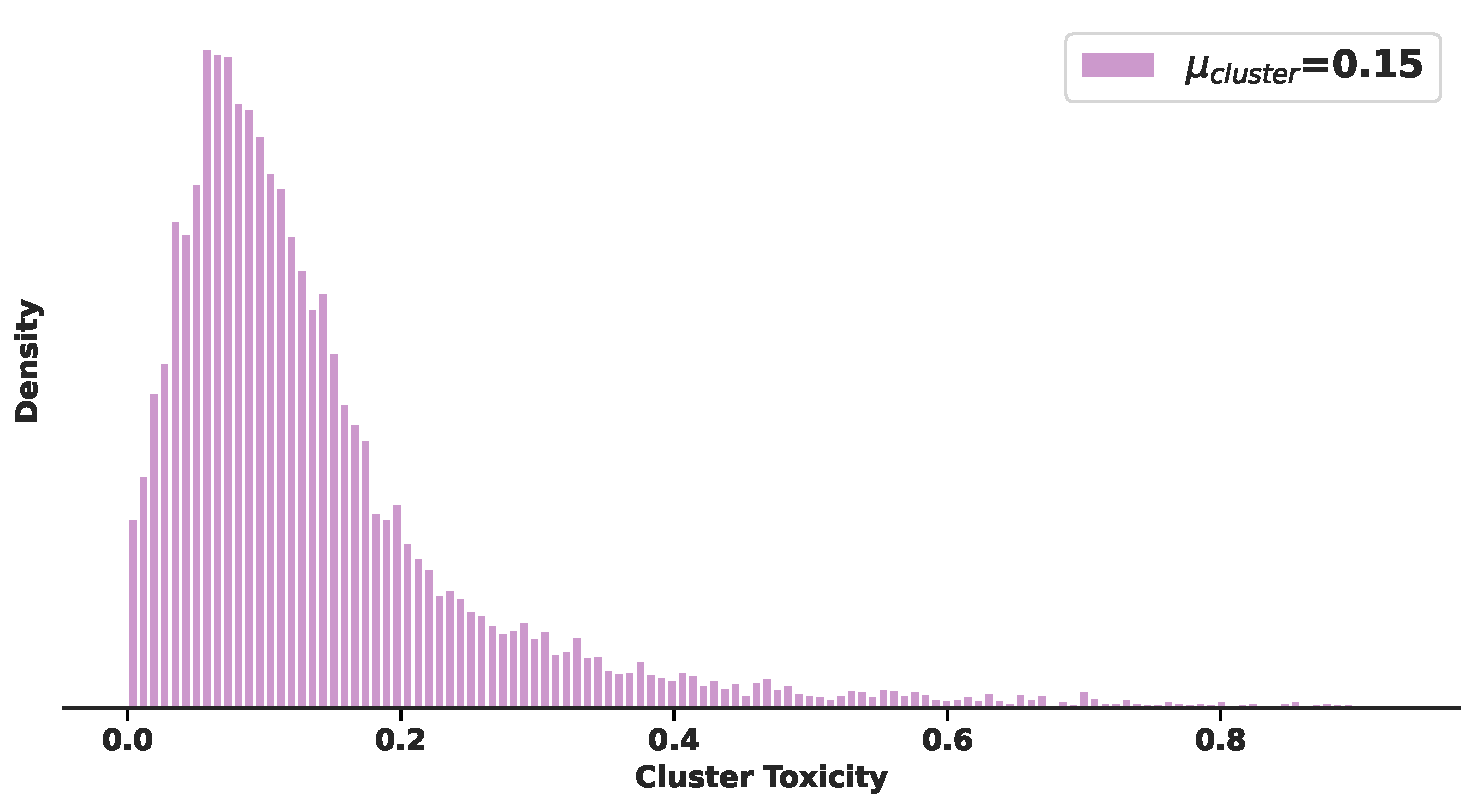
\includegraphics[width=1\columnwidth]{figures/cluster_toxicity_dist3.pdf}
\caption{}
\label{fig:cluster-dists-toxic}
\end{subfigure}
\begin{subfigure}[l]{0.45\textwidth}
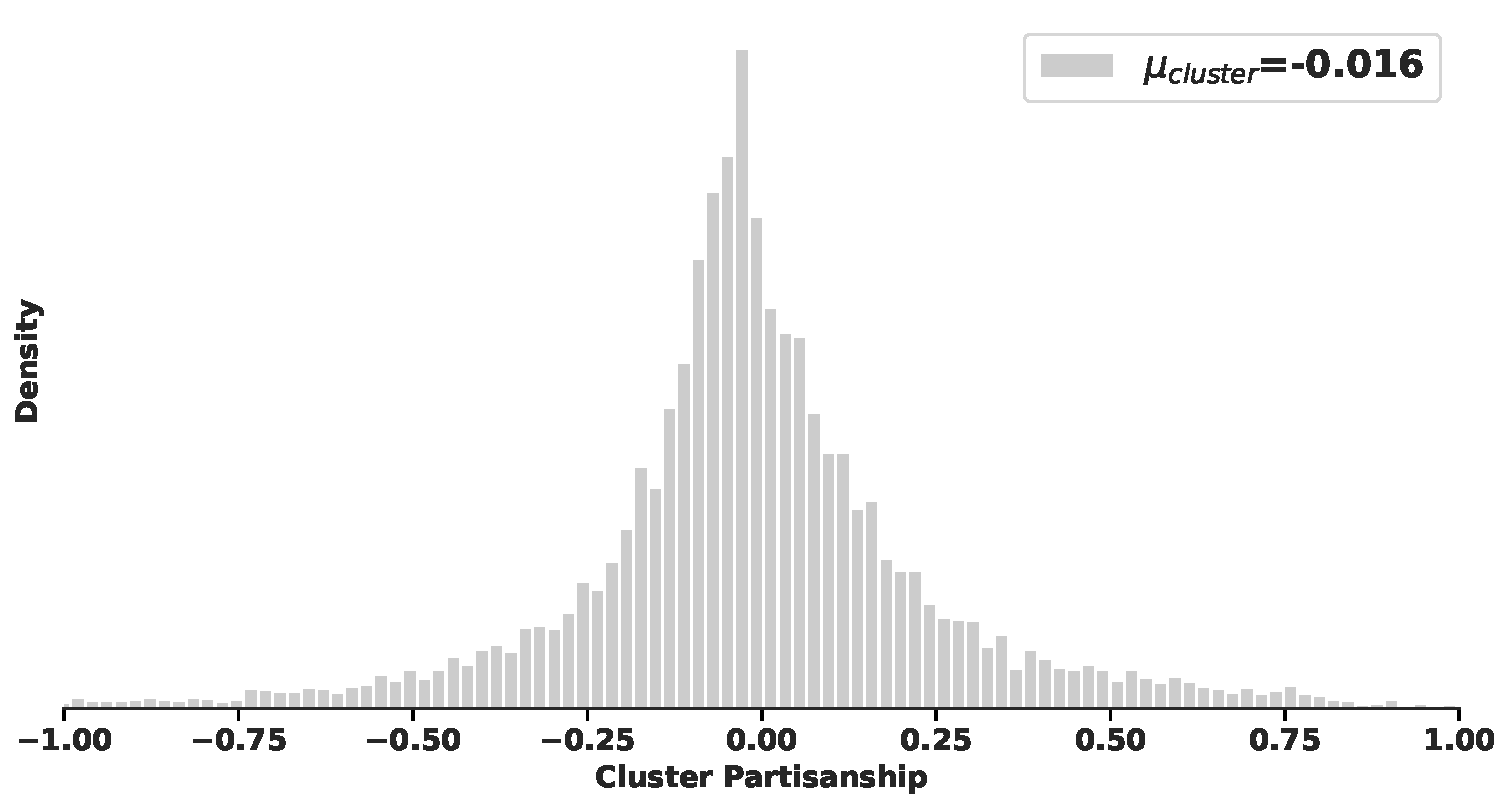
\includegraphics[width=1\columnwidth]{figures/cluster_partisanship_dist3.pdf} 
\caption{}
\label{fig:cluster-dists-part}
\end{subfigure}
\caption{The distribution of toxicity and partisanship within our set of clusters.}
\end{figure}

\vspace{2pt}\noindent
\noindent
\textbf{Estimating the Toxicity of Topics.}
To estimate the toxicity of particular topics, we determine the average toxicity score of all tweets present within that given cluster. While we largely rely on our average toxicity scores, in addition to this metric, we further determine the \emph{percentage} of toxic tweets within our \emph{entire} English-language dataset that conforms to that particular topic.  Namely, after identifying each toxic cluster center, for each of these toxic cluster centers, we further identify the set of non-toxic tweets that also conform to the topic. We then calculate the percentage of toxic tweets (\textit{i.e.}, toxicity > 0.5) per topic. 

To assign non-toxic tweets to our set of toxic tweet centers, we utilize the approach laid out in prior work~\cite{hanley2022happenstance,hanley2023partial} and subsequently assign each non-toxic tweet to the cluster center with the highest semantic similarity to the tweet. As recommended by Hanley {et~al.}~\cite{hhanleyspecious2024}, given our fine-tuned version of MPNet, we again utilize a cluster threshold of 0.60 for assigning a given non-toxic tweet to a given cluster. We plot the distribution of estimated topic toxicity in Figure~\ref{fig:cluster-dists-toxic}. We utilize this approach, rather than clustering all 89.6 million English tweets given the size of our dataset, and because, for this work, we largely are only concerned with topics that have some level of toxicity. 

\vspace{2pt}\noindent
\noindent
\textbf{Estimating the Partisanship of Topics.}
To further examine the role of partisanship within interactions within particular topic clusters, we further determine the overall political orientation of each cluster. To do so, after assigning all remaining non-toxic tweets to our clusters as specified above, we subsequently determine which set of users participated/tweeted about that topic. Calculating the average and standard deviation of the political orientations of all the Twitter users (utilizing our previous calculations of user partisanship [Section~\ref{sec:background-ca}]) that tweeted about that topic, we thus estimate each topic's political-ideological composition. We plot the distribution of the partisanship of our set of clusters in Figure~\ref{fig:cluster-dists-part}. 


\subsection{The Most Toxic Topics of 2022\label{sec:most-toxic}}

\begin{table*}
\centering
\scriptsize
\selectfont
\setlength{\tabcolsep}{4pt}
\begin{tabularx}{\textwidth}{lXrrrXrrr}
\toprule
 &   &  &   \# Toxic & Avg.& Example & Avg.  & Avg. Partisan  & Partisan \\
 Topic& {Keywords}&\# Tweets &Tweets  & Toxicity &  Tweet  & Partisan. & of Toxic Users& Std. \\
\midrule
 1 & biden, joe, administration, president, senile  &246,868 & 39,102 (15.84\%) & 0.1824& Joe Biden And everything is screwed up. You suk & 0.642 &0.379 &1.084\\ 

 2 & ukraine, russia, kyiv, putin, independent &763,153 & 36,425 (4.77\%) &0.070 &  So l guess you what Ukraine to stop fighting back and let the Russians kill them. Ukraine Will Resist Fuck Putin& -0.091 &0.031 & 0.899\\ %\hline

3 & lie, pathological, truth, habitual, liar  &100,825 & 26,894 (26.67\% ) &0.298 & These leftist serial liars always project onto others the crimes they are perpetrating. & -0.055 & 0.081 & 1.0300  \\

 4 & party, democrat, republican, dnc, destroying &111,763 & 22,705 (20.32\%) &0.232 & That slate is FAR better than the gaggle of corrupt Marxists the racist lunatic democrat party pushed forward. Nobody is gonna give you a nod for badmouthing the better team.
  &0.215&  0.171 & 1.162\\

  
 5& ballot, election, stolen, voting, rigged& 295,356 &  22,399 (7.58\%) &0.093 & You already know that the Maricopa County Election will say "Fuck Your Ballots" and ram it through the certifications.& 0.199 & 0.121 & 1.131 \\

  6 & fox, news, murdoch, carlson, tucker & 179,224 & 20,958 (11.69\%) &0.138 &Fox News Give it a rest already. For is even worse than national enquirer for false made up trash. & -0.027 & 0.089 & 1.116 \\

  7 & filipkowski, ron, flynn, bannon, nut & 107,255& 19,018 (17.73\%)&0.187 & @REDACTED Man are Fox ppl nuts or what &-0.686 & -0.535 & 0.784  \\

  8 & tweet, follow, deleted, algorithm, account & 190,665 & 18,822 (9.87\%)  &0.102& Ok is anybody else's twitter completely fucked up and glitchy?
 & 0.044 &  0.038 & 0.982\\

  9 & stupidity, smart, intelligent, educated, dumb & 23,232 & 18,533 (79.77\%)&0.688 &@I mean how stupid are these people or what?
What happened to like history classes?
Gees what a bunch of loser white people.&  0.141 &  0.131 & 0.938 \\

  10 & abortion, birth, pro-life, pregnancy, fetus &309,723 & 18,456 (5.96\%)&0.087& This moron thinks the Supreme Court literally edited the Bill of Rights to remove the right to an abortion. Dumb as fucking rocks these people.
 &  0.114 &.112 & 1.265 \\

\bottomrule
\end{tabularx}
\caption{Top toxic topics---by the number of toxic tweets---in our dataset.\label{table:toxic-topics}} 
\end{table*}
We start this section by providing an overview of the topics with the most toxic tweets in 2022 (Table~\ref{table:toxic-topics}). We further give an overview of the most partisan topics in Appendix~\ref{sec:partisan-toxic} and the most toxic topics in Appendix~\ref{sec:most-toxic-by-percentage} (most of these topics are merely users calling each other different epithets). As seen in Table~\ref{table:toxic-topics}, many of the most common toxic tweets concerned the most politically divisive issues of 2022~\cite{Montanaro2022}, namely, Joe Biden's administration (Topic 1;~246,968K tweets), Russia's invasion of Ukraine (Topic 2;~763K tweets), and the abortion rights in the United States in the wake of the Dobss v. Jackson decision which overturned US federal abortion rights~\cite{StaffAborrtion2022}.

Examining the average partisanship of the user who tweeted about each of the top toxic topics, we find distinct political differences. Markedly, we observe, that those who tweeted in a toxic manner about the Ukraine War tended to have a slight rightward tilt (+0.122 rightward tilt). Examining these tweets, we find right-leaning users when tweeting about the war, excoriated or derided the Ukrainian government or military, which was picked up as toxic by our contrastive-DeBERTa model. 
For example, one ``toxic'' tweet by a rightward user stated: 
\begin{displayquote}
\small
\textit{
No more arms for a Ukraine refusing to negotiate! Ukraine doesn't need more arms, Ukraine needs more intelligence! And Zelensky is a dictatorial asshole!}

\end{displayquote}
In contrast, considering all users who tweeted about the war, we find that they tended to lean leftward (-0.091 leftward tilt) with one left-leaning user tweeting:
\begin{displayquote}
\small
\textit{
Stand With Ukraine!}
\end{displayquote}
Looking at the users who tweeted about Joe Biden's presidency (Topic~1),  we again see a rightward bias (+0.642) among users who tweeted about him or his administration generally and with users who tweeted about him in a toxic manner (+0.379). For example, one user tweeted
\begin{displayquote}
\small
\textit{
Save the poor water bottle from that pedophile Joe Biden before he becomes a victim}
\end{displayquote} We thus observe that those talking about the administration (both in a toxic and non-toxic manner) were largely right-leaning (as largely expected given that the Biden administration is Democratic). Finally, examining the set of users who tweeted about abortion in 2022 (Topic~10), we again find a rightward lean among users who tweeted about this issue. For example, one right-wing user wrote:
\begin{displayquote}
\small
\textit{Why are actors so ignorant about policies? States can still do abortions. Go ahead and murder more babies.}
\end{displayquote}



Besides these politically salient issues, we observe several topics where politically charged users simply derided each other (Topic~4), called each other idiotic (Topic~9), or called the other political side liars (Topic~3). We further see in Topic~5 heavy emphasis on the US presidential election being stolen in Arizona. As documented by Prochaska et~al., a misinformation story called Sharpiegate where ``Sharpies invalidated ballots in Maricopa County, Arizona'' was widely spread on Twitter and we see evidence of it in our dataset with several political users heatedly and toxically calling the Arizona election rigged~\cite{prochaska2023mobilizing}.





\subsection{Topic Dependent Changes in Partisanship and Toxicity \label{sec:changes}} Having explored some of the most prominent toxic topics during our period of study, we now explore how the toxicity of different Twitter topics change as users of different political orientations enter and leave. We find that regardless of whether a topic moderates (\textit{i.e.}, political orientation moves closer to 0) or becomes more extreme (\textit{i.e.}, political orientation becomes more left-leaning or more right-leaning), on average, this movement has little bearing on toxicity. Indeed correlating the change in the political orientation of a given topic between January and December with the percentage change in the toxicity of that conversation, we calculate a Pearson correlation of $\rho=-0.0168$, indicating little to no relationship. Similarly, we find that the variance of political participation in particular topics over time is also only slightly correlated with the toxicity of a given topic $\rho=-0.098$. This indicates that unlike for users, a different dynamic may be influencing the toxicity of particular topics across time. 

Across our dataset, we find that regardless of whether the topic moderates or moves to the extremes, in both cases, toxicity generally increases (55.8\% of the time for topics that moderated in partisanship and 71.4\% of the time for topics that moved to the political extreme). Furthermore, we find that between January 2022 and December 2022, in 34.8\% of topics, as topics became more right-leaning, they also became more toxic; in 27.1\% cases, they became less toxic as they became more right-leaning. Conversely, in 21.2\% of our topics, they became more toxic as they became more left-leaning, and in  17.0\% of topics they became less toxic as they became more left-leaning. However, examining each cluster, we \emph{do} find that on a cluster-by-cluster basis as the political composition of users involved in that topic changes there are corresponding changes in toxicity.

\begin{figure}
\begin{subfigure}[l]{0.32\textwidth}
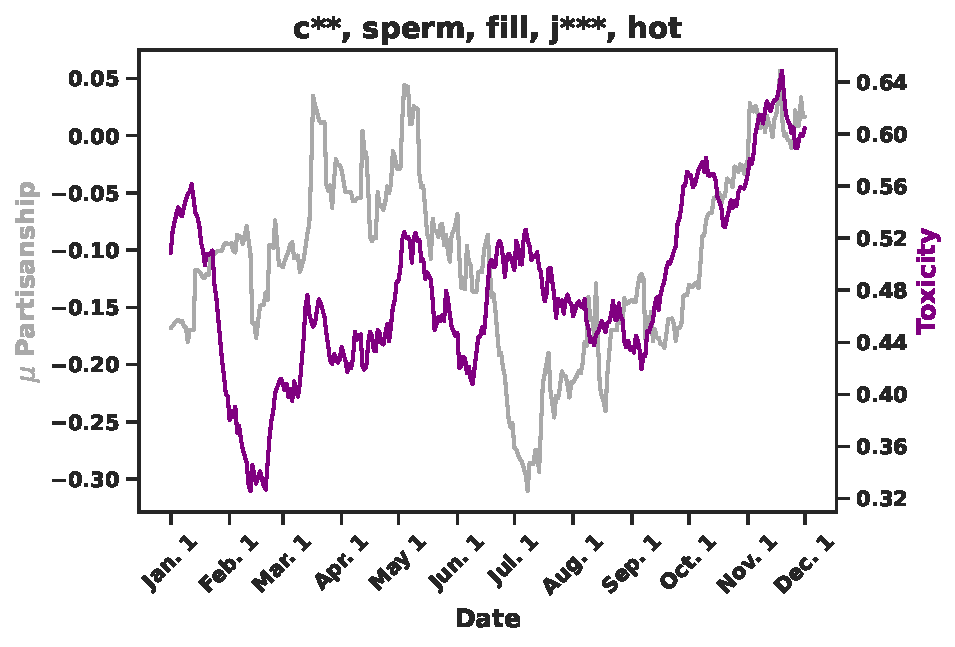
\includegraphics[width=1\columnwidth]{figures/c__-toxic-swing-final-20240425.pdf} 
\caption{}
\label{fig:cum}
\end{subfigure}
\begin{subfigure}[l]{0.32\textwidth}
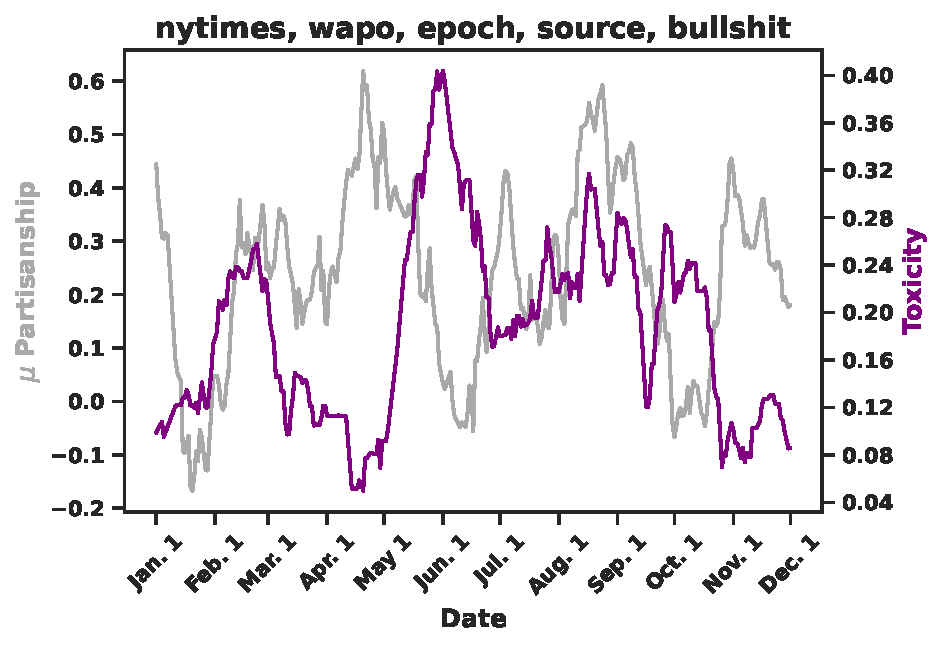
\includegraphics[width=1\columnwidth]{figures/nytimes-toxic-swing-final-20240425.pdf} 
\caption{}
\label{fig:nytimes}

\end{subfigure}
\begin{subfigure}[l]{0.32\textwidth}
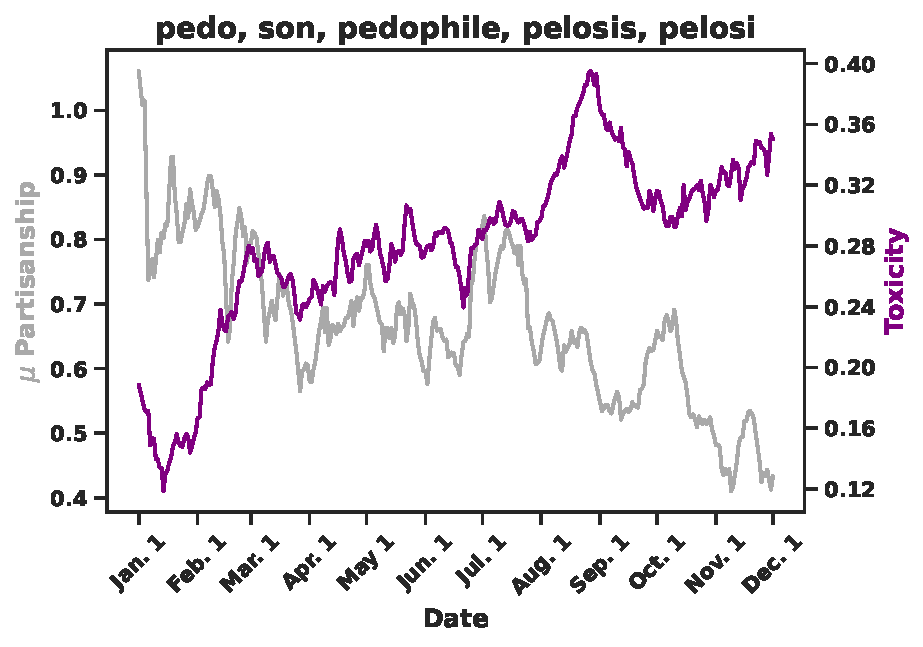
\includegraphics[width=1\columnwidth]{figures/pedo-toxic-swing-final-20240425.pdf} 
\caption{}
\label{fig:pedo}
\end{subfigure}
\begin{subfigure}[l]{0.32\textwidth}
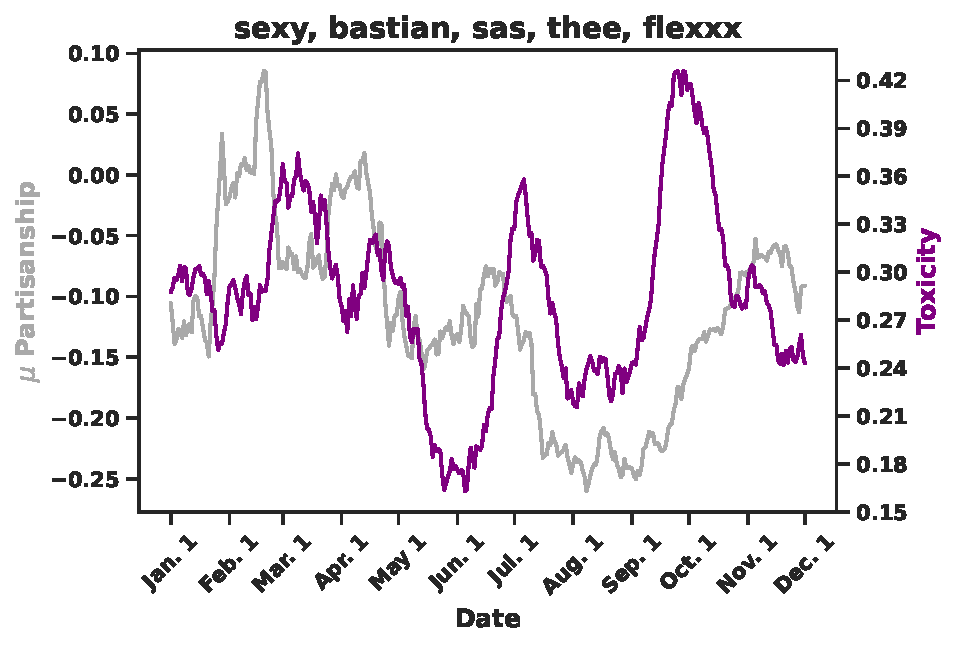
\includegraphics[width=1\columnwidth]{figures/sexy-toxic-swing-final-20240425.pdf} 
\caption{}
\label{fig:sexy}
\end{subfigure}
\begin{subfigure}[l]{0.32\textwidth}
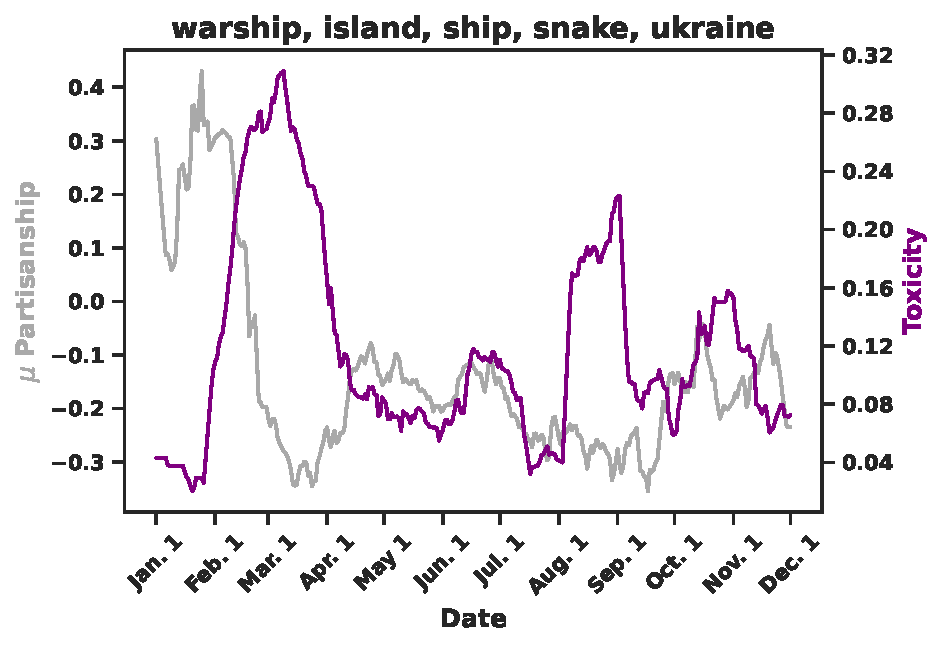
\includegraphics[width=1\columnwidth]{figures/warship-toxic-swing-final-20240425.pdf} 
\caption{}
\label{fig:warship}
\end{subfigure}
\begin{minipage}[l]{1\textwidth}
\caption{Topics with the largest increase in toxicity in 2022. \label{fig:toxicity-swing}}
\end{minipage}
\vspace{-15pt}
\end{figure}



\begin{figure}
\begin{subfigure}[l]{0.32\textwidth}
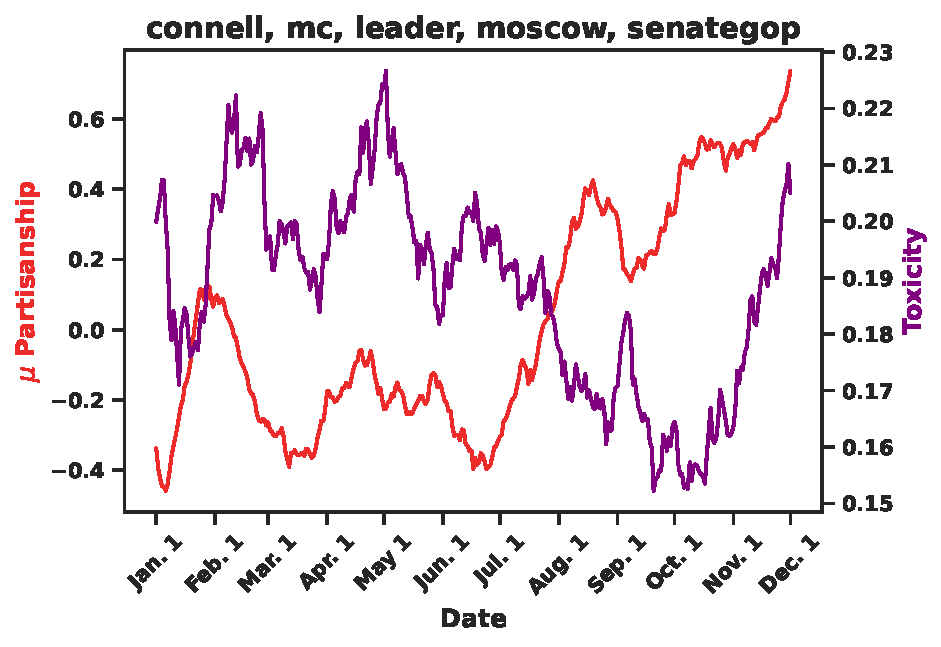
\includegraphics[width=1\columnwidth]{figures/connell-conservative-final-20240425.pdf} 
\caption{}
\label{fig:moscow}
\end{subfigure}
\begin{subfigure}[l]{0.32\textwidth}
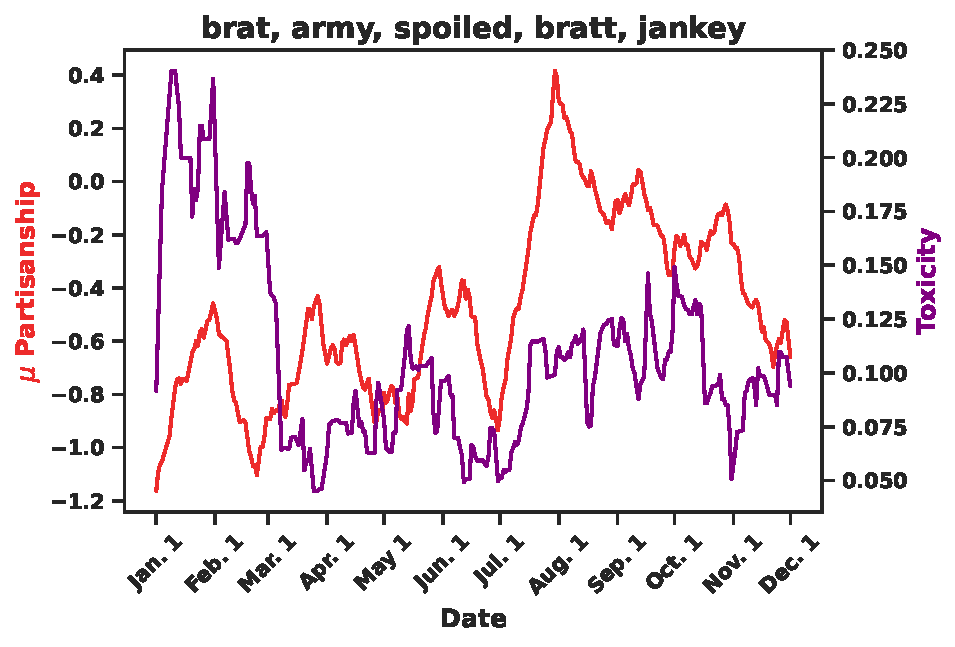
\includegraphics[width=1\columnwidth]{figures/brat-conservative-final-20240425.pdf} 
\caption{}
\label{fig:brat}
\end{subfigure}
\begin{subfigure}[l]{0.32\textwidth}
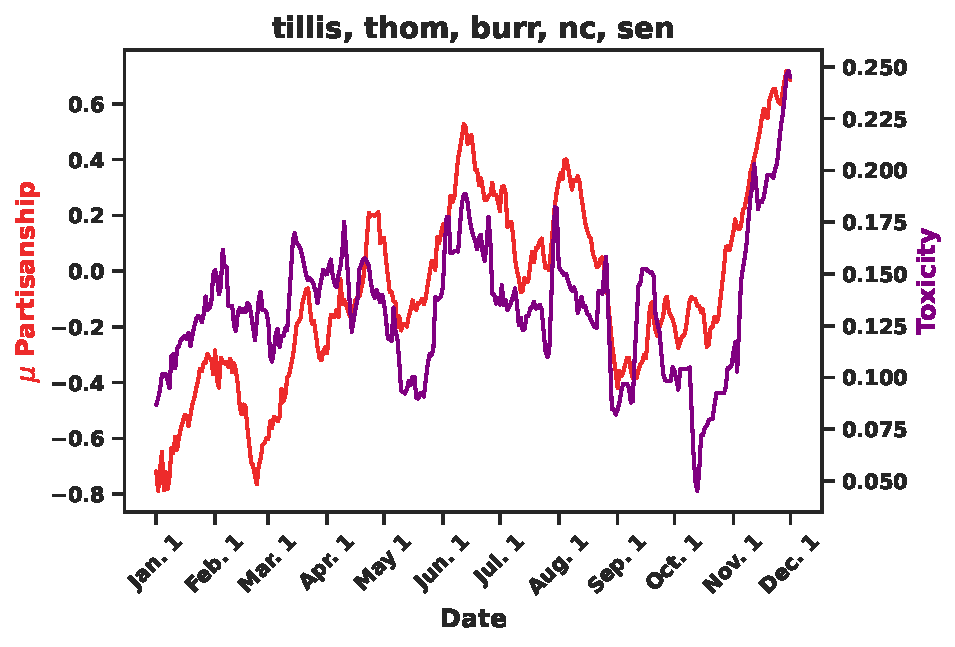
\includegraphics[width=1\columnwidth]{figures/tillis-conservative-final-20240425.pdf} 
\caption{}
\label{fig:tillis}
\end{subfigure}
\begin{subfigure}[l]{0.32\textwidth}
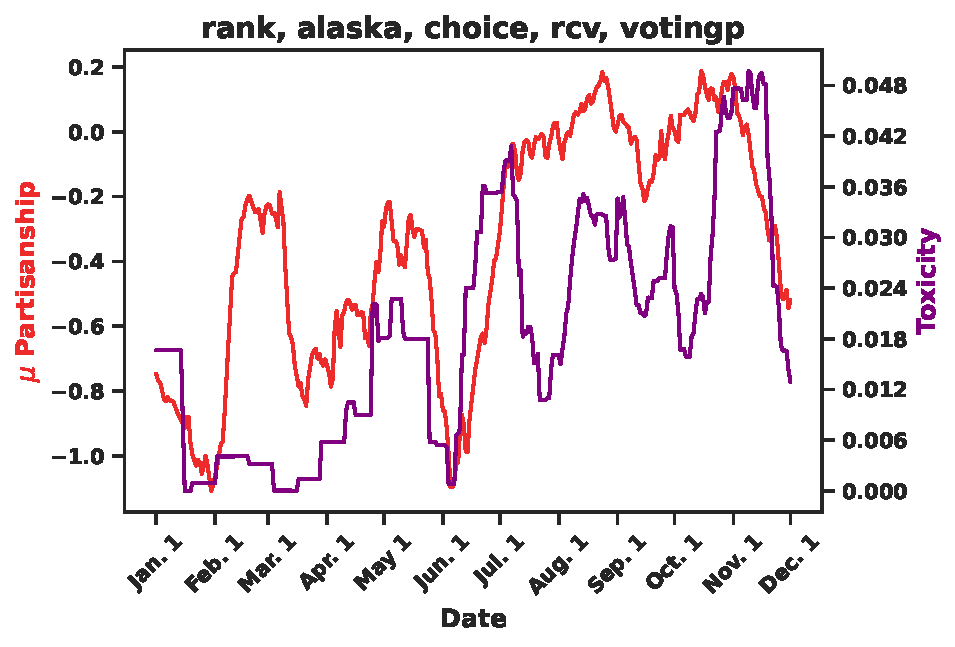
\includegraphics[width=1\columnwidth]{figures/rank-conservative-final-20240425.pdf} 
\caption{}
\label{fig:rank}
\end{subfigure}
\begin{subfigure}[l]{0.32\textwidth}
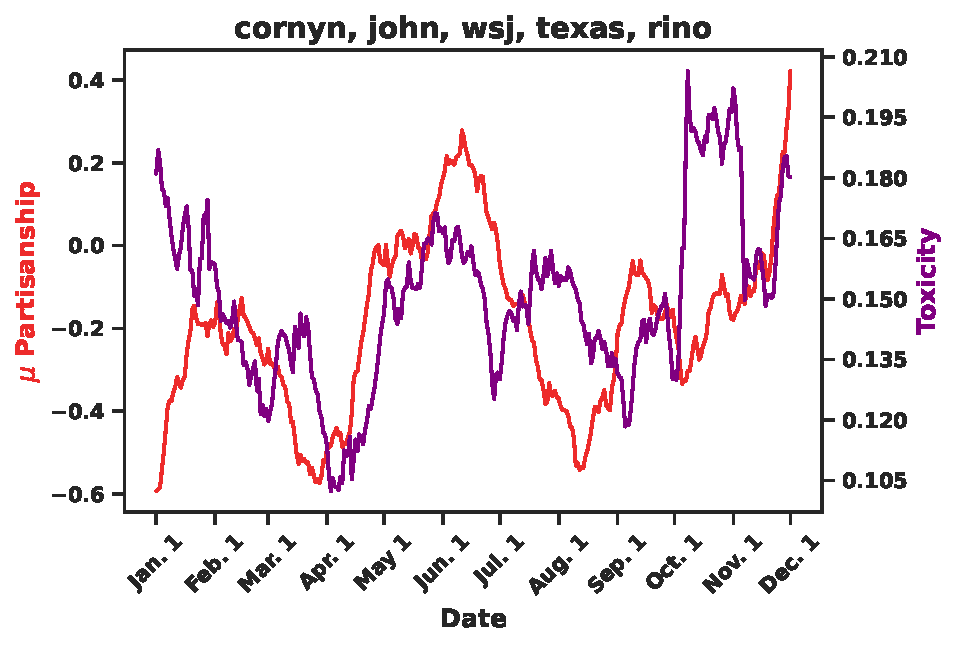
\includegraphics[width=1\columnwidth]{figures/cornyn-conservative-final-20240425.pdf} 
\caption{}
\label{fig:cornyn}
\end{subfigure}
\begin{minipage}[l]{1\textwidth}
\caption{Topics with the largest swing to right-leaning partisanship throughout 2022. \label{fig:conservative-swing}}
\end{minipage}
\end{figure}


\vspace{2pt}
\noindent
\textbf{Toxic Swings.} To further qualitatively understand the nature of how toxicity and political orientation change over time, we plot the toxicity and partisanship for the topics with the largest increases in toxicity between January 2022 and December 2022. We observe that while for four topics considered, (Figures~\ref{fig:cum},~\ref{fig:nytimes},~\ref{fig:sexy}, and~\ref{fig:warship}) as the topic became more right-leaning, toxicity similarly increased, for one of the topics (Figure~\ref{fig:pedo}), we observe the opposite. Examining, each we observe, noticeable trends where, depending on the political nature of the topic,  a corresponding swing in the political composition of the users in the left or the right direction, is correlated with an increase in toxicity. For instance, in the tweets surrounding the New York Times and the Washington Post's accuracy,  we observe that as users discussing the topic became more right-leaning, the more toxic the tweets. We similarly find for the topic surrounding the destruction of Russian warship on Snake Island by Ukrainians, the more right-wing the users, the more toxic. For example, one user wrote:
\begin{displayquote}
\small
\textit{
    Surprising Russian Navy Losses Against Ukraine Century After Tsushima 
Ukraine is really FUCKING Russian Navy Ship's up during the Russian Invasion into Ukraine}
\end{displayquote}

\noindent
In contrast, for Topic 3 (Figure~\ref{fig:pedo}), we observe that as users became more left-leaning the overall toxicity of the topic decreased. We observe that this is largely due to left-leaning users adopting retorts to right-leaning users calling the Democratic former Speaker of the House Nancy Pelosi a pedophile. For example, we observe one user stating:

\begin{displayquote}
\small
\textit{
Let's not forget that the last republican speaker of Michigan house was a Pedophile who raped a 15 year old sister in law.}
\end{displayquote}

\noindent
We thus observe among these top topics that depending on the political nature of the given topic and how users are interacting and replying to other users about the topic, a corresponding swing in the political composition of the users in the opposite direction, may or may be correlated with an increase in toxicity. 



\noindent
\vspace{2pt}
\textbf{Left-Leaning and Right-Leaning Swings.} Plotting the set of topics with the largest swings in average political orientation, to both the right and left-leaning end, between January 2022 and December 2022 (Figures~\ref{fig:conservative-swing} and~\ref{fig:liberal-swing}), we again observe that changes in toxicity as a result of these changes are largely dependent on the topic. For example, as the conversation surrounding Tom Tills (the senior Republican Senator for North Carolina) became more right-leaning, the toxicity of that topic increased dramatically (Figure~\ref{fig:tillis}). Despite Senator Tillis being a Republican, we observe that this is largely due to right-leaning users largely labeling Senator Tillis a RINO (Republican in name only) with one user posting:

\begin{displayquote}
\small
\textit{You've always been a RINO
NC must be ashamed of you}
\end{displayquote}
\noindent We find a similar behavior for Senator John Cornyn of Texas, again with a user writing:

\begin{displayquote}
\small
\textit{John Cornyn This Bill is trash. RINOs need to go.
Cornyn votes with the Democrats almost as often as his own party.
Texas should be ashamed}
\end{displayquote} We similarly find that as right-leaning users joined the conversation about US Senate Republican Minority Leader Mitch McConnell being beholden to the Russian government~\cite{Hulse2018} toxicity increased. We note that the attacks against Senators Mitch McConnell, John Cornyn, and Tom Tillis were \emph{all} largely for not being conservative enough. Finally, for Democratic Manhattan District Attorney Alvin Bragg, we also observe that when more right-leaning users joined the conversation surrounding him, toxicity increased. However, unlike for the Republican Senators, more intuitively, this was largely due to his investigation of former Republican President Donald Trump. 

In contrast, for Republican Ohio Governor Mike DeWine, we observe that as more left-leaning users joined the conversation surrounding him the topic became more toxic, with one user writing
\begin{displayquote}
\small
\textit{
Gov Mike DeWine Thank you, Gov Mike DeWine, for making it easier for Ohioans to be killed by gun violence. Fuck you.}
\end{displayquote}
Similarly, for Republican Florida Congressman Matt Gaetz, we also observe that as more liberal users joined the discussions surrounding him the topic became more toxic. We find that this was largely sparked by a tweet from Matt Gaetz stating:

\begin{displayquote}
\small
\textit{Over-educated, under-loved millennials who sadly return from protests to a lonely microwave dinner with their cats, and no bumble matches.}
\end{displayquote}
\noindent to which one user replied 
\begin{displayquote}
\small
\textit{Only stupid, insecure men worry about women being over-educated. Which one are you, matt gaetz?}
\end{displayquote}

\noindent
We thus observe that the context of each of these topics, in particular, is decisive for determining how different swings in political polarization will affect the overall toxicity of the topic. As within individual users (See Section~\ref{sec:toxic_middle}), partisanship itself does not necessarily predict a higher degree of toxicity within conversations but is largely topic-dependent. Even the target/topic being a right-leaning or left-leaning entity/individual not decisively giving whether a left or right-leaning shift in users will correspond to an increase in toxicity. 

\begin{figure}
\begin{subfigure}[l]{0.32\textwidth}
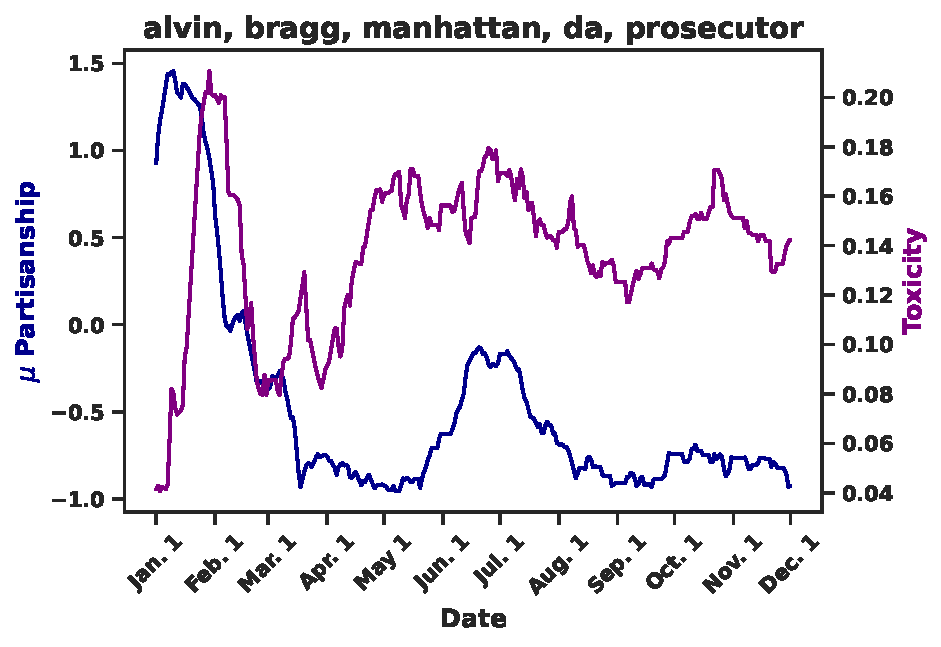
\includegraphics[width=1\columnwidth]{figures/alvin-lib-final-20240425.pdf} 
\caption{}
\label{fig:alvin}
\end{subfigure}
\begin{subfigure}[l]{0.32\textwidth}
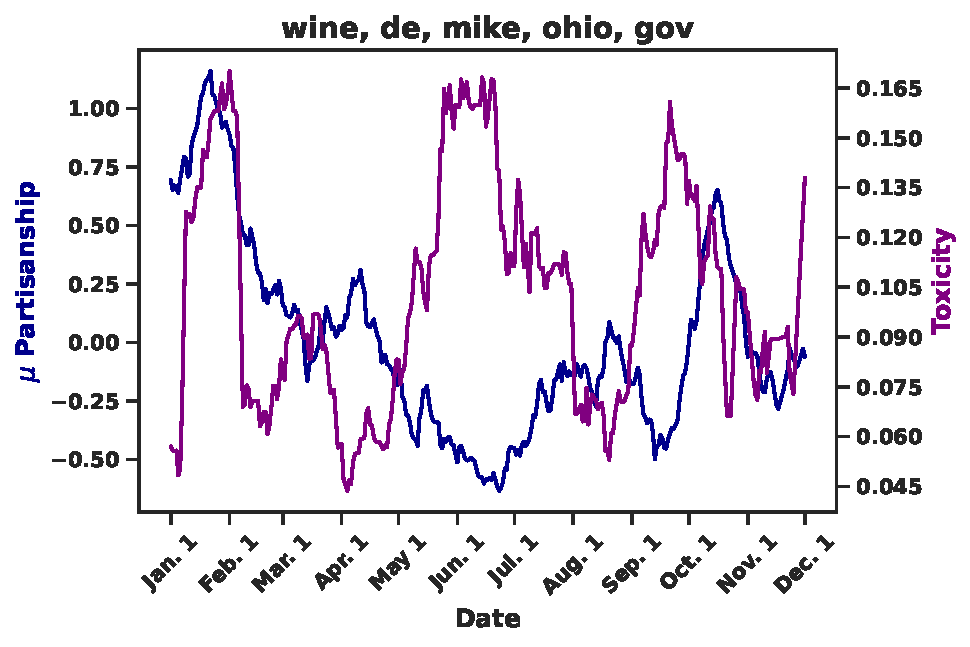
\includegraphics[width=1\columnwidth]{figures/wine-lib-final-20240425.pdf} 
\caption{}
\label{fig:wind}
\end{subfigure}
\begin{subfigure}[l]{0.32\textwidth}
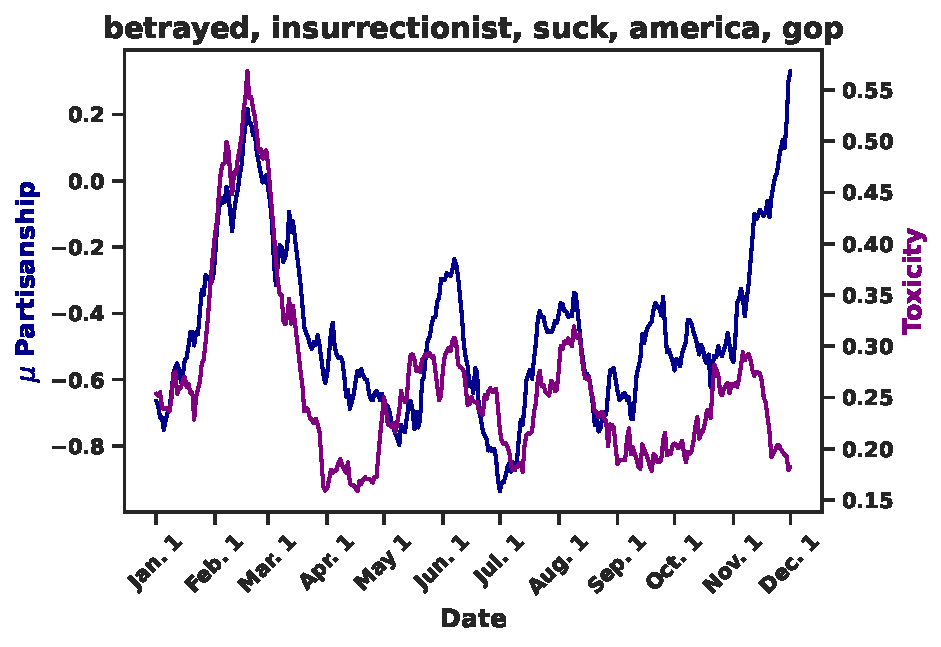
\includegraphics[width=1\columnwidth]{figures/betrayed-lib-final-20240425.pdf} 
\caption{}
\label{fig:betrayed}

\end{subfigure}
\begin{subfigure}[l]{0.32\textwidth}
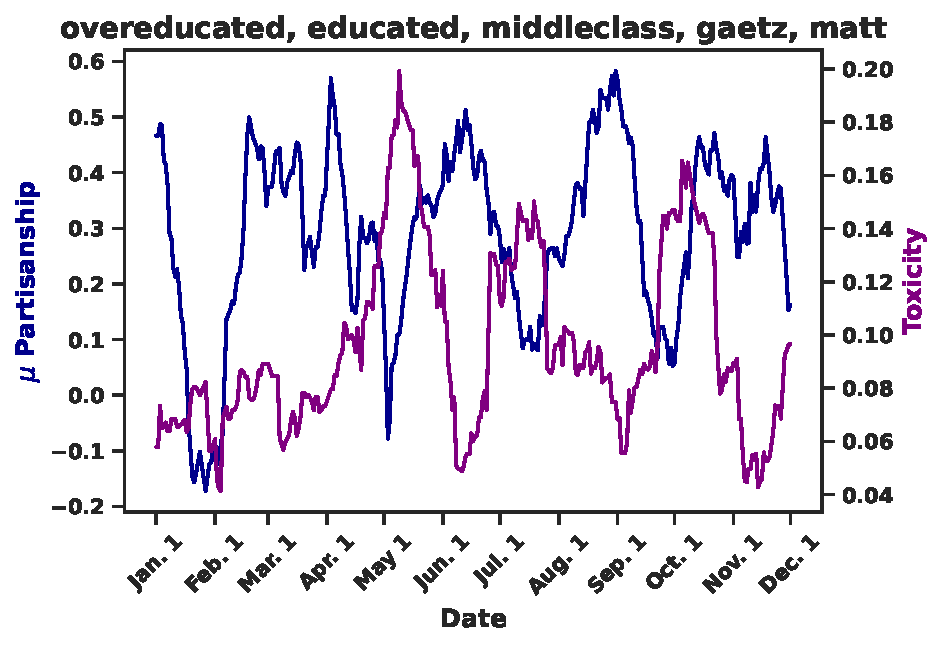
\includegraphics[width=1\columnwidth]{figures/overeducated-lib-final-20240425.pdf}
\caption{}
\label{fig:overeducated}
\end{subfigure}
\begin{subfigure}[l]{0.32\textwidth}
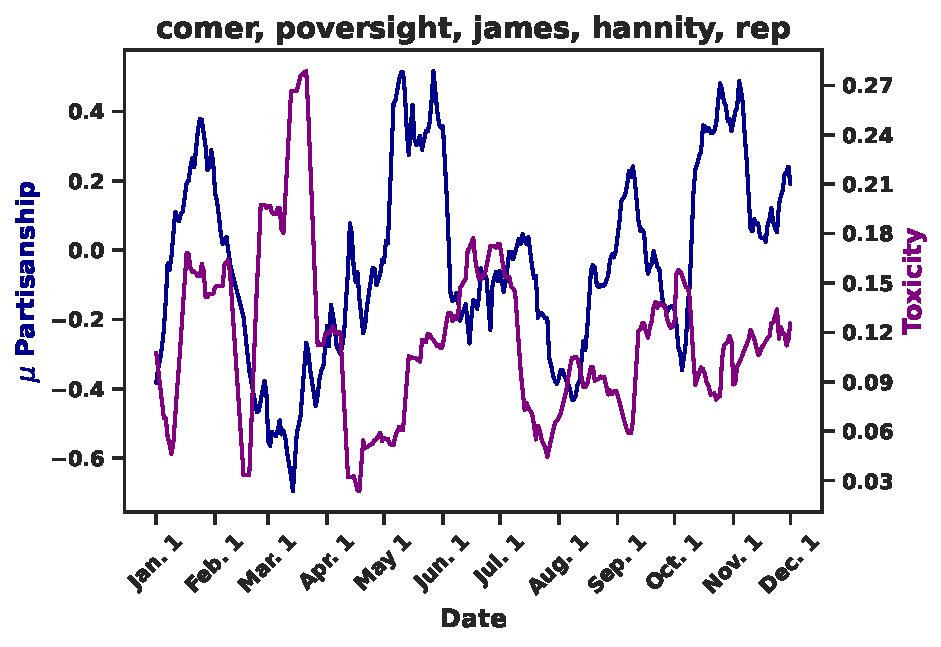
\includegraphics[width=1\columnwidth]{figures/comer-lib-final-20240425.pdf} 
\caption{}
\label{fig:comer}
\end{subfigure}


\begin{minipage}[l]{1\textwidth}
\caption{Topics with the largest swing to left-leaning partisanship throughout 2022. \label{fig:liberal-swing}}
\end{minipage}

\end{figure}

\subsection{Topic User Composition and the Toxicity of Topics\label{sec:topic-level-gam}} Having qualitatively described the composition and changing dynamics of some of our set of topic clusters, we now determine how the several user-level features of individual topic clusters predict the toxicity within the topic to better understand what may be influencing the toxicity of individual topics.

We note, and as seen throughout this section, topics on Twitter vary widely with individual topics often varying widely in political composition over time. Across all topics considered in our dataset, on average between January 2022 and December 2022, the political composition of the users tweeting about each topic changed by 0.159 standard deviations (based on the latent space that we previously determined [Section~\ref{sec:background-ca}]). In 61.9\% of cases, topics became more right-leaning, and in 38.1\%  topics became more left-leaning; similarly, within this same period, 56.0\% became more toxic while 44.0\% became less toxic. As a result, to quantify the effect that the composition of users has on the toxicity of a given topic at a single point in time, for each topic and each month combination, we gather the user compositions and the cluster characteristic data. We thus, in this section seek to determine the factors that determine the average toxicity score of a topic within a single month time-span. 

As before, to determine the role of various topic-level features in the overall toxicity of that cluster, we fit a GAM on the average toxicity score each month within each of our clusters against: \begin{enumerate}
    \item \emph{The number of users who tweeted about that topic.}
    \item \emph{The average user toxicity in the cluster.}
    \item \emph{The percentage of users involved in that topic that is Twitter verified.}
    \item \emph{The average of the partisanship in that cluster.}
    \item \emph{the standard deviation of political ideologies of users within that topic cluster.}
    \item \emph{The average age of the users in clusters.}
\end{enumerate}

Again, as in Section~\ref{sec:toxic_middle} when fitting our model, we perform variable selection based forward selection based on the Akaike Information Criterion~\cite{akaike2011akaike} Furthermore, again, to ensure that our model generalizes, we reserve out 10\% of our data as validation, and in our results report our model's $R^2$ value on this validation set. After fitting this regression, we further determine the estimated importance of each variable to our final model by permuting the features and seeing the estimated impact on the $R^2$ score of the validation set of our data. We do not consider other user account characteristics due to their multicollinearity with user toxicity (as seen in Section~\ref{sec:toxic_middle}, many user characteristics are correlated with their individual toxicity). Finally, we again reproduce our results with the Perspective Toxicity API in Appendix~\ref{sec:cluster-perspective-tox} obtaining similar results.


\begin{figure}
\begin{minipage}[l]{1.0\textwidth}
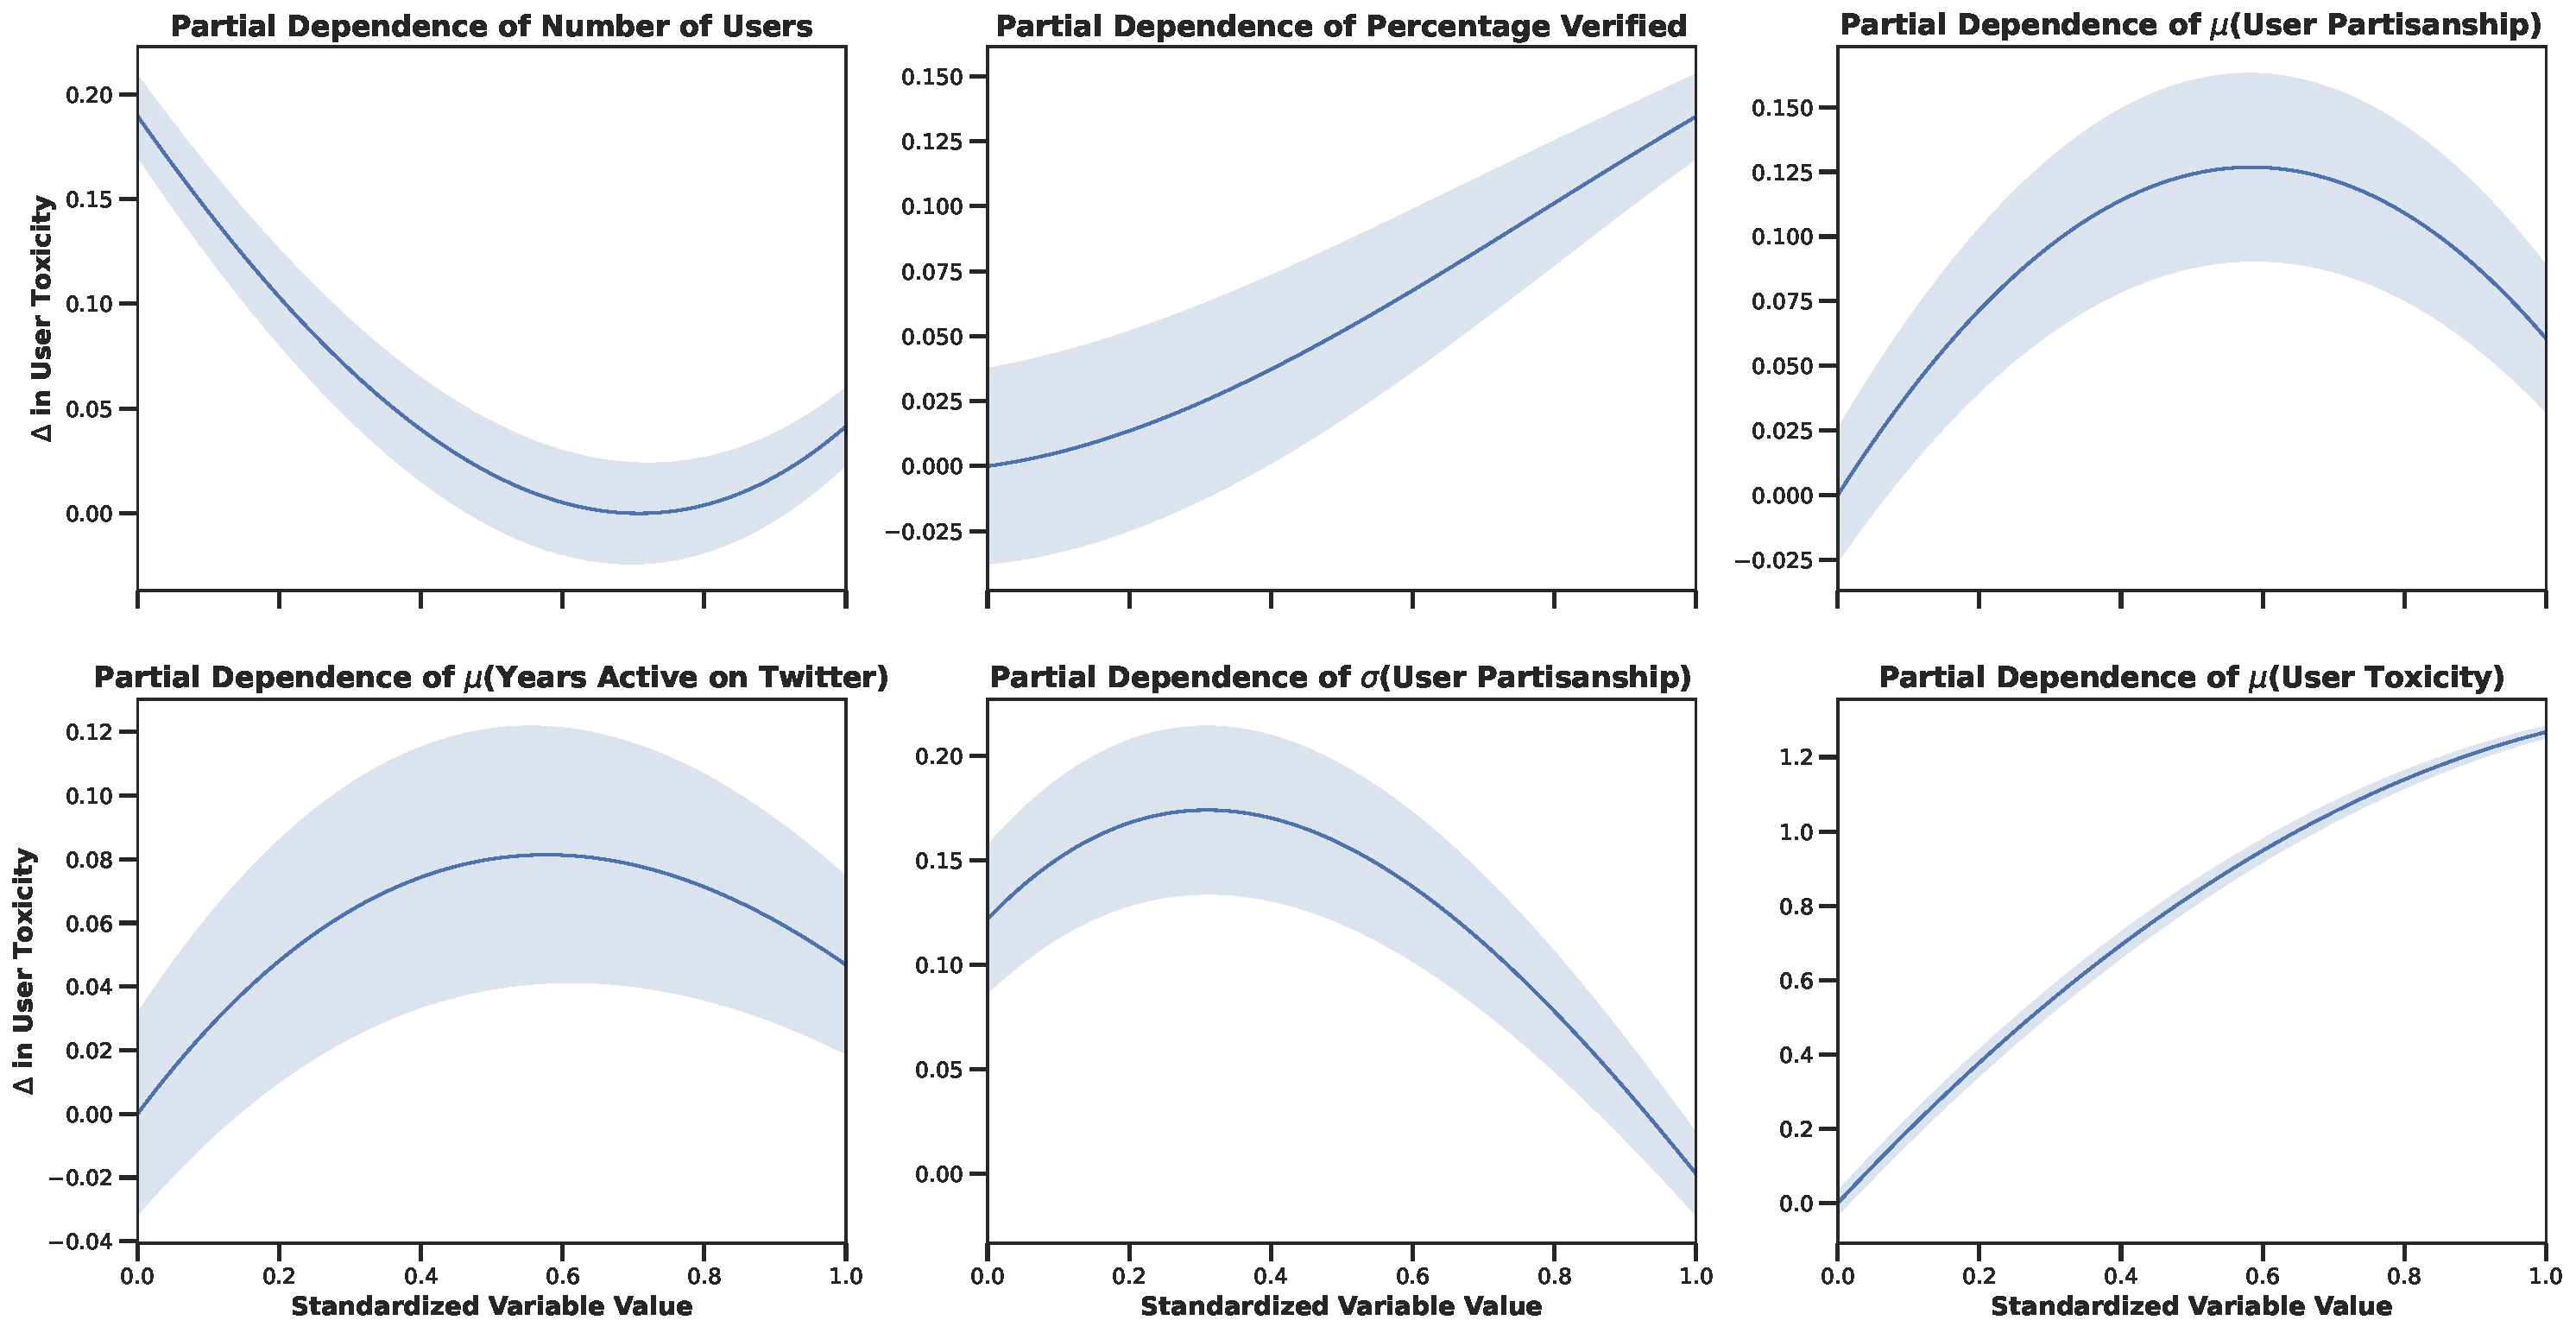
\includegraphics[width=1\columnwidth]{figures/partial_dependence_important_variables-clusterlevel-1.pdf} 
\end{minipage}
\begin{minipage}[l]{1\textwidth}
\caption{Partial dependencies with 95\% Normal confidence intervals between our fitted standardized dependent variables and cluster toxicity.}
\label{fig:partial-dependcies-clusterlevel}
\end{minipage}

\end{figure}

\begin{table}
    \small
    \centering
    \begin{tabularx}{0.85\columnwidth}{l|rrr}
     Train $R^2$: 0.397, Validation $R^2$:  0.389  \\
    \toprule
      Dependent Variable  & Pearson Corr. $\rho$ & Kendall's $\tau$ & Permut Import. \\    \midrule
  Number of Users &-0.292 & -0.139  & 0.445  \\
 $\mu$(Years Active on Twitter) &-0.191 & -0.186 & 0.018\\
  Percentage Verified &0.234 & 0.250 & 0.007  \\
$\sigma$(User partisanship) & 0.098 & 0.003 & 0.021 \\
  $\mu$|User partisanship) & 0.028 &  0.005 & 0.007 \\
  $\mu$(User Toxicity) &  0.589 & 0.486 & 0.502 \\
    \bottomrule

    \end{tabularx}
  \caption{Pearson correlation $\rho$ and Kendall's $\tau$ of dependent variables and clusters' toxicities. } 
   \vspace{-15pt}
   \label{table:regression-clusterlevel}
\end{table}




As seen in Table~\ref{table:regression-clusterlevel}, and Figure~\ref{fig:partial-dependcies-clusterlevel}, unsurprisingly, the most important factor in determining the toxicity of a given topic is the toxicity of the users contributing tweets to the cluster. This one variable has a permutation importance of 0.50 and a correlation of 0.58 with the toxicity of a given cluster. Simply put, unsurprisingly, topics whose corresponding users have higher average toxicity are more likely to have toxic content. As in Section~\ref{sec:toxic_middle}, we again observe being further along the political spectrum does not necessarily indicate increased toxicity and that a conversation being dominated by right-leaning or left-leaning users has little bearing on its toxicity. 

We find, as seen in Figure~\ref{fig:partial-dependcies-clusterlevel}, that the number of users involved in a given topic appears to have a moderating and mitigating effect on the toxicity of that topic ($\rho=0.292$). This also appears as one of the most important features for determining the average toxicity with a permutation score of 0.445. However, conversely having more verified individuals participating in that topic \emph{does} increase toxicity. We thus find (from Section~\ref{sec:toxic_middle}) that while verified users are less likely to tweet toxic content, their presence and their tweeting about particular topics correlate with increased toxicity in that topic. We further find that despite the average age of accounts participating in a topic having a negative Pearson correlation in our fitted model if the average age of the accounts participating in a conversation is very young or much older, there is a decreased toxicity compared to topics that engage accounts of all ages.

Examining political ideological contributions in Figure~\ref{fig:partial-dependcies-clusterlevel}  to the toxicity of individual topics we find that topics dominated by all left-leaning or all right-leaning users are largely the least topics compared to topics in the middle of the ideological spectrum. Finally examining the partial dependence of the diversity of viewpoints that participate in a given topic at a given point in time, we find that while initially the greater the political diversity of the topic cluster, the more toxic it becomes, as the topic invites more and more users of different beliefs that the topic cluster decreases in toxicity. While further research is needed, this result reinforces the work of Mamkos et~al. that find that for particular typically non-political topics that engage users from all over the political spectrum, these topics tend to be less toxic than others~\cite{mamakos2023social}.

 \begin{figure}
\begin{minipage}[l]{0.6\textwidth}
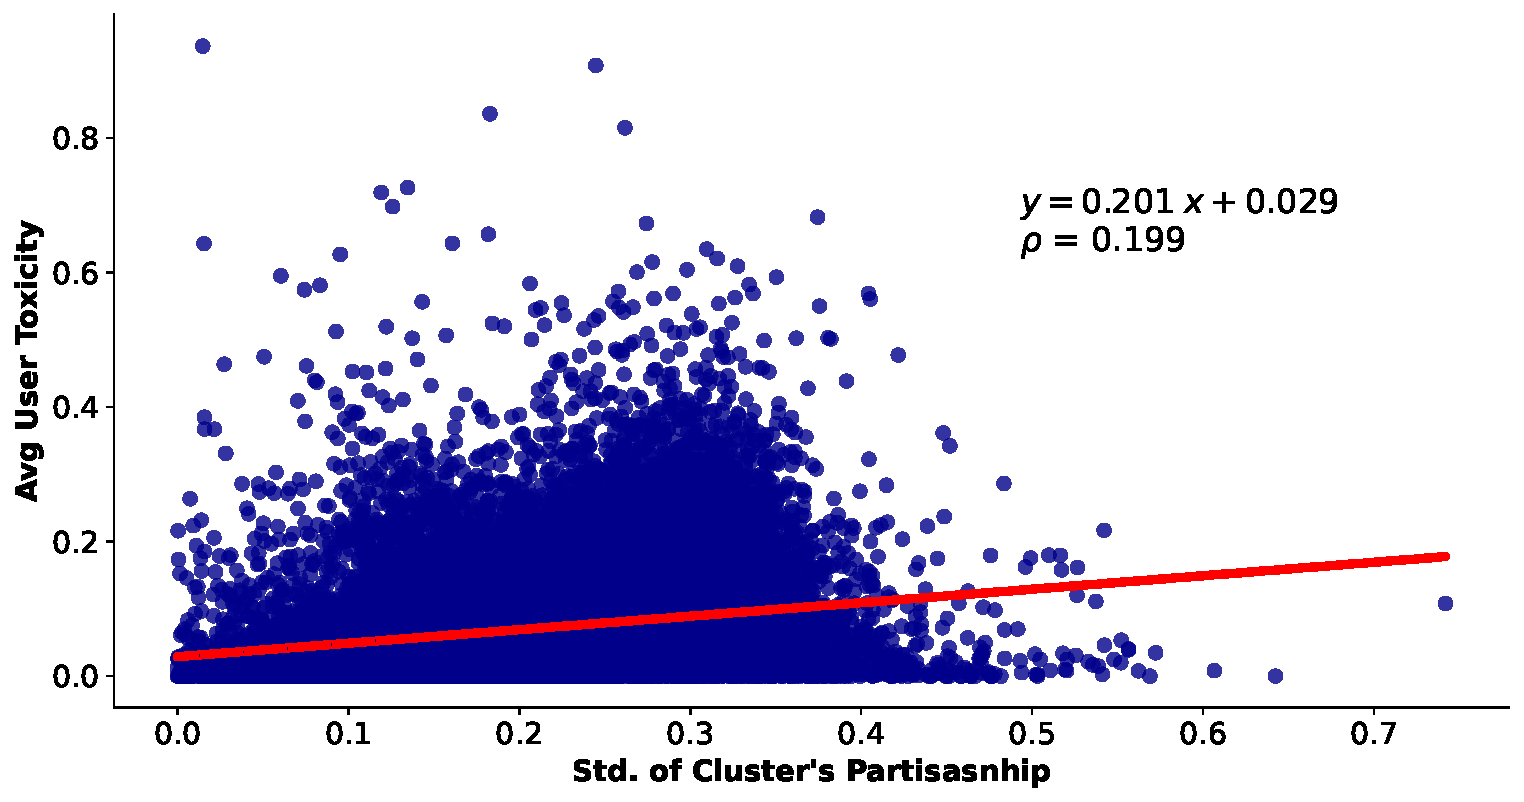
\includegraphics[width=1\columnwidth]{figures/cluster_user_ideology_vs_user_toxicity-20240429.pdf} 
\end{minipage}
\begin{minipage}[l]{0.33\textwidth}
\caption{As previously also found in our analysis of user characteristics (Section~\ref{sec:calculated}), we find that as users engage in a wider window of topics of particular political ideologies, the more toxic their tweeted content\label{fig:toxicity-vs-var-user}}
\end{minipage}

\end{figure}


Lastly, looking in the reverse direction, we determine how users' toxicity changes when they are involved in many different types of politically aligned topics.  As also found by Mamkos et~al.~\cite{mamakos2023social}, we find, as seen in Figure~\ref{fig:toxicity-vs-var-user},  as users are involved in a higher variance of topics of different political orientations their average toxicity increases ($\rho=0.19$). We thus find from this analysis further confirmation, on a topic level, that increased user toxicity and the diversity of views present in a given conversation contribute to toxicity within particular topics. However, conversely, as topics invite a wider range of individuals into a discussion toxicity actually decreases. We now consider some of the implications of these results. 









